%     Pacotes e configurações padrão do estilo "article"\ -------------------------------------
\documentclass[a4paper,11pt]{article}
%     Layout --------------------------------------------------------
\newcommand{\tituloCapa}{Estudo Processos Interativos} 
\title{\tituloCapa}
%     Gráficos e layout ----------------------------------------------------------------------
\usepackage[T1]{fontenc}
\usepackage[utf8]{inputenc}
%\usepackage{lmodern}
\usepackage{times} % fonte Times New Roman
%     Pacotes adicionados -------------------------------------------------------------------
\usepackage{ae}
%     Língua e hifenização ------------------------------------------------------------------
\usepackage[brazilian]{babel}
\usepackage{hyphenat}
% ---------------------------------------------------------------------------------------
\usepackage{fancyhdr}
\usepackage{sectsty}
\usepackage{float}
%\usepackage{graphicx}
\usepackage[pdftex]{color,graphicx}
\usepackage{verbatim}
\usepackage[pdftex]{hyperref}
\usepackage[nottoc]{tocbibind}
\usepackage{amsthm}
\usepackage{enumerate} % Permite alterar Layout do enumerate
\usepackage{pdflscape} % Permite alterar a orientação da pagina
\usepackage{ifthen} % Permite usar condicionais ifelse
\usepackage[table]{xcolor} % Permite alterar as cores das celulas de uma tabela
\usepackage{amsmath} % Ambiente para uso de elementos matemáticos
%\usepackage{gnuplottex} % permite usar diretamente o gnuplot
%     Dados do título e autores --------------------------------------------------------------
%\title{\tituloRelatorio}
\author{Rafael Lima}
%     Definições do pdf ----------------------------------------------------------------------
\hypersetup{
    unicode=false,          % non-Latin characters in Acrobat’s bookmarks
    pdftoolbar=true,        % show Acrobat’s toolbar?
    pdfmenubar=true,        % show Acrobat’s menu?
    pdffitwindow=false,     % window fit to page when opened
    pdfstartview={FitH},    % fits the width of the page to the window    
    pdfauthor={Rafael Lima},     % author
    %pdfkeywords={} {} ,    % list of keywords
    pdfnewwindow=true      % links in new window
}
% Layout do documento ------------------------------------------------------------------------
 \pagestyle{fancy}
%     Cabeçalho e Rodapé ---------------------------------------------------------------
      \lhead{}
      \chead{}
      \rhead{}
      \lfoot{}
      \cfoot{}
      \rfoot{\thepage}
      %     Númeração ------------------------------------------------------------------------
      \pagenumbering{arabic}
      %     Retas do cabeçalho e rodapé ------------------------------------------------------
      \renewcommand{\headrulewidth}{0.5pt}
      \renewcommand{\footrulewidth}{0.5pt}
      %     Tamanho da letra de seções e derivadas --------------------------------------------
      \sectionfont{\normalsize}
      \subsectionfont{\small}
      %     Hiperlinks ------------------------------------------------------------------------
      \hypersetup{
                  colorlinks,
                  citecolor=black,
                  filecolor=black,
                  linkcolor=black,
                  urlcolor=black
                  }
%     Outros ----------------------------------------------------------------------------
      \addto\captionsbrazilian{\renewcommand{\contentsname}{Índice}} % Muda nome dos contents
      %\renewcommand{\thesection}{(\alph{section})} % muda o estilo de númeração das sections
      % alterando a formatação dos numeradores de lista de itens
      \renewcommand\theenumi{\arabic{enumi}}
	  \renewcommand\labelenumi{(\textit{\theenumi})}
	  \renewcommand\theenumii{\arabic{enumii}}
	  \renewcommand\labelenumii{(\textit{\theenumi.\theenumii})}
      
% ---------------------------------------------------------------------------------------

\hypersetup{pdftitle={\tituloCapa}}    % title
%     Definições Auxiliares -----------------------------------------
%% compilar com lualatex

%% \luaTable{'numDeColunas'}{'nomeArquivo.dat'}{'legenda'}
%% {'linha de Titulo'}

\begin{luacode}
  numC = 3

  function readfileDat(filename)
    local filename = "../data/"..filename

    for line in io.lines(filename) do
        local numl = {}
        for n in string.gmatch(line,"[\%d\%.]+") do
          numl[#numl+1] = tostring(n)
        end
        numC = #numl -- rever esta parte
        tex.sprint(table.concat(numl," & ")," \\\\");
    end
  end
\end{luacode}

\newcommand{\luaTable}[4][\directlua{tex.print(numC)}]
{
  \begin{table}[H]
  \centering
  \caption{#3}
  \begin{tabular}{*{#1}{c}}
  \hline
  #4\\
  \hline
  \directlua{readfileDat('#2')}
  \hline
  \end{tabular}
  \end{table}
}

% Exemplo de uso:
% \luaTable[3]{teste.dat}{legenda}{x&y&z}

% -----------------------------------------------------------------

\begin{luacode}
  function readEquationTex(vecEq)
    -- TODO verificar problemas para valores 3, 5 e 10
    local texEq = {}

    for _,eq in ipairs(vecEq) do
      local texfile = io.open(table.concat({'pol','.tex'},eq),'r')
      texEq = texfile:read("*all")
      tex.sprint(table.concat({eq,texEq},' & ')," \\\\")
    end

    tex.sprint(tableEq)
  end
\end{luacode}

\newcommand{\polyTable}[3][tbPoly]
{
  \begin{table}[H]
    \label{#1}
    \centering
    \caption{#3}
    \begin{tabular}{l p{10cm}}
      \hline
      $i$ & $f_i(x)$\\
      \hline
      \directlua{readEquationTex({#2})}
      \hline
    \end{tabular}
  \end{table}
}

%% Exemplo de uso \eqTable{1,3,5,10}{Polinômios gerados}

% ----------------------------------------------------------------- 

\newcounter{cGraph}
\setcounter{cGraph}{1}
\newcommand{\plotedFigure}[2][\value{cGraph}]{
  \begin{figure}[H]
    \centering
    \includegraphics[width=8cm]{../image/graph#1.png}
    \caption{#2}
  \end{figure}
  \stepcounter{cGraph}
}
% % para acionar scripts
%-------------------------------~>ø<~--------------------------------
\begin{document}
% Capa e Índice -----------------------------------------------------
%--------------------------------------------------- Capa --------------------------------------------
\newpage
\begin{flushleft}
    {UNB - Universidade de Bras\'ilia\\}
    {MAT - Departamento de Matem\'atica\\}
    {Disciplina: C\'alculo Numérico\\}
    {Professor: Yuri Durmaresq Sobral\\}
\end{flushleft}
      \vspace{6.0cm}
      \begin{center}
      {\Huge \tituloCapa}
      \end{center}
      \vspace{8.0cm}
      
 \begin{tabular}{ll}
 \textit{Aluno} & \textit{Matr\'icula}\\
 Di\'ogenes Oliveira & 10/0009972\\
 Felipe Bressan & 11/0116593\\
 Rafael Lima & 10/0131093\\
 \end{tabular}
%\thispagestyle{empty} % Retira o cabeçalho e o rodapé da página

% ------------------------------- Índice ---------------------------
\newpage
%\tableofcontents
%\newpage
% ---------------------------------------------------------------------------------------

% Mapa Logístico ----------------------------------------------------
\section{Mapa logístico}

\paragraph{Questão 1}Temos que o processo é dado por $x_{n+1} = \lambda\cdot x_n\cdot (1-x_n)$. Se $x*$ é um ponto que não se altera ao longe do processo temos que:
$$x* = \lambda \cdot x*\cdot(1-x*)$$
\begin{equation}
x* = \{0,1 -\frac{1}{\lambda}\}
\end{equation}
\paragraph{}Analizando-se o processo, observa-se que para valores inteiros positivos de $x_0$ o processo se encaminha para zero e para os demais valores reais positivos o processo tende a $$x* = 1 -\frac{1}{\lambda}$$. De modo que espera-se que para um valor alto de $\lambda$ o processo tenha ponto fixo próximo de $1$.

\paragraph{Questão 2}Aplicando-se o processo para vários valores de $lambda$ observa-se o seguinte comportamento:
\begin{figure}[H]
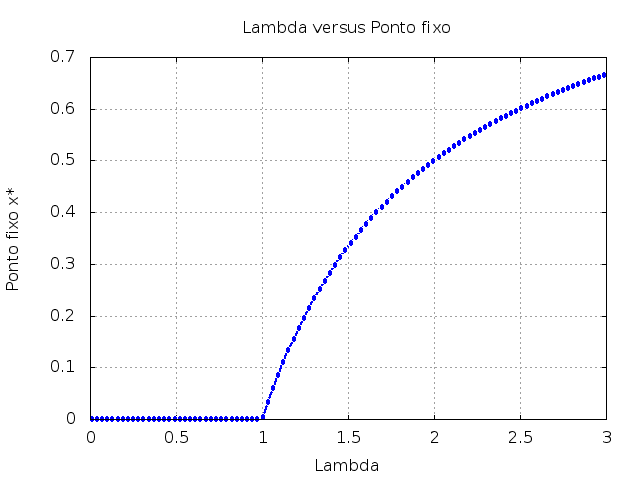
\includegraphics[width=11cm]{../image/questao2a.png}
\centering
\caption{Gráfico de $\lambda$ vs $x^*$}
\end{figure}

\paragraph{}Nota-se que para $\lambda$ entre 0 e 3, como ilustrado a função tem somente um ponto fixo:
\begin{figure}[H]
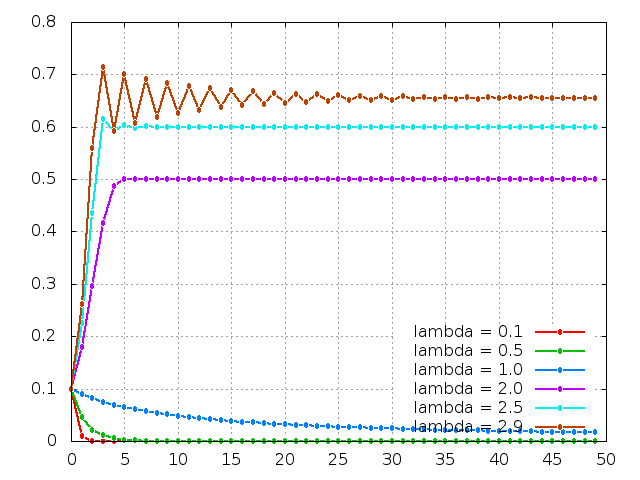
\includegraphics[width=11cm]{../image/questao2b1.png}
\centering
\caption{Gráfico de $x_n$ vs $n$ para $0<x_0<3$}
\end{figure}

\paragraph{}Para valores maiores que 3 e menores que 4 de $\lambda$ temos que a função diverge oscilando entre valores compreendidos entre 0 e 1:

\begin{figure}[H]
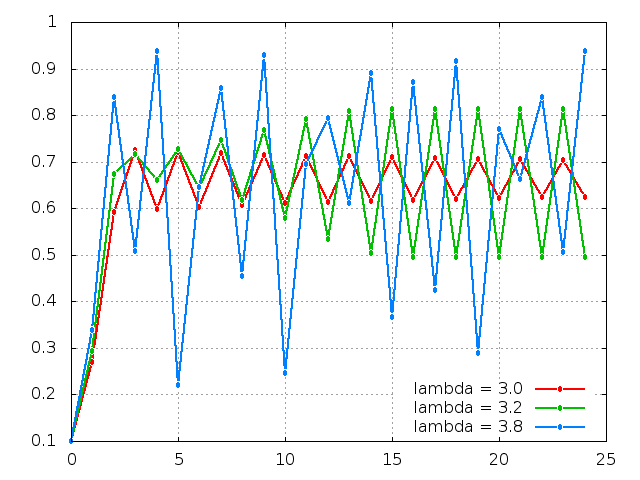
\includegraphics[width=11cm]{../image/questao2b2.png}
\centering
\caption{Gráfico de $x_n$ vs $n$ para $3<x_0$}
\end{figure}

\paragraph{}Aumentando um pouco mais o valore de $lambda$, temos que a o processo não mais tem pontos fixos, tendendo a $-\inf$:

\begin{figure}[H]
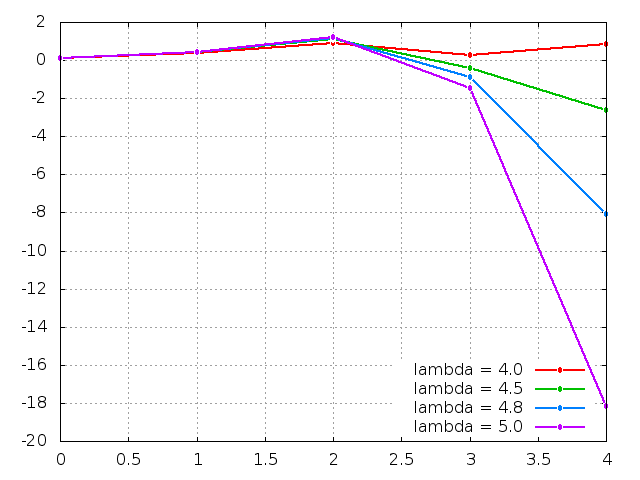
\includegraphics[width=11cm]{../image/questao2b3.png}
\centering
\caption{Gráfico de $x_n$ vs $n$ para $4<x_0$}
\end{figure}

\paragraph{Questão 3}
\paragraph{}Com base no mesmo processo, obteve-se que para valores de $\lambda$ que 3 o processo apresenta o comportamento ilutratado no gŕafico:
\begin{figure}[H]
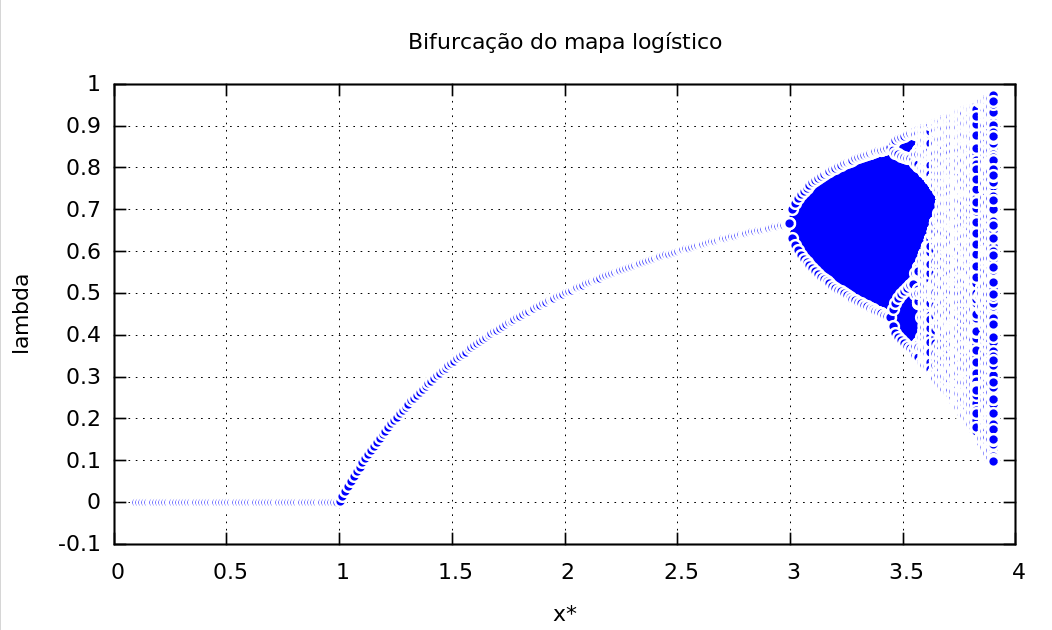
\includegraphics[width=11cm]{../image/questao3b.png}
\centering
\caption{Gráfico dos valores das orbitas de x* para cada valor de $\lambda$}
\end{figure}

\paragraph{Questão 4}
\paragraph{}A partir do estudo do período, obtive-se que para $x_0 = 0.1$, no programa atual temos que:
\begin{table}[H]
\centering
\begin{tabular}{cc}
\hline
Maior período & 4409\\
Orbita de periodo 2 & 2467\\
Orbita de periodo 5 & 164\\
\hline
\end{tabular}
\end{table}
\begin{figure}[H]
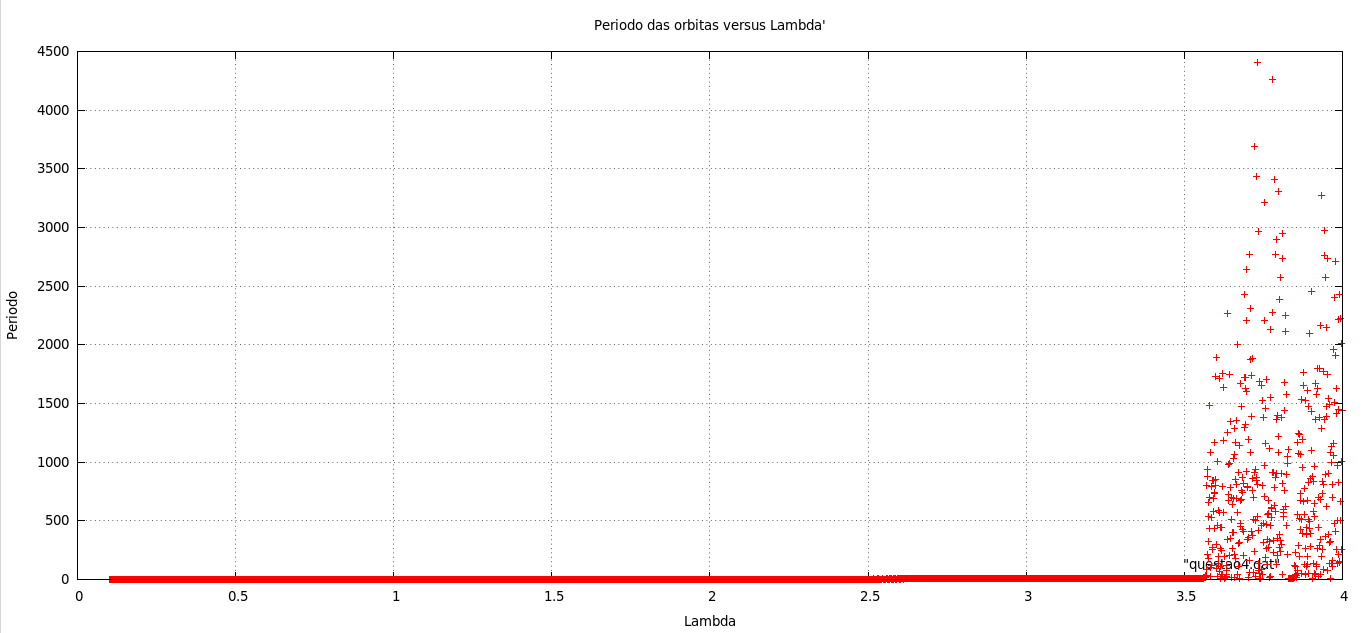
\includegraphics[width=11cm]{../image/questao4.png}
\centering
\caption{Gráfico dos periodo das orbitas vs $\lambda$}
\end{figure}

% Propagação do calor numa barra -----------------------------------
\section{Propagação do calor numa barra semi-infinita}
\paragraph{Questão 5}Podemos encontrar a temperatura de uma barra semi-infinita em um posição $x$ e um instante $t$ através da expressão
\begin{equation}\label{eqTemp}
T(x,t) = T_i + q\left[2\sqrt{\frac{\alpha t}{\pi}e^{-\frac{x^2}{4\alpha t}}} - x\cdot erfc\left( \frac{x}{2\sqrt{\alpha t}}\right)\right]
\end{equation}
em que a função $erfc(x)$ é a função erro complementar, definida como:
\begin{equation}\label{eqErfc}
erf(z) = \frac{2}{\sqrt{\pi}}\int_{z}^{\inf}{e^{-w^2}dw}
\end{equation}
\paragraph{}Através do qual podemos contruir um processo interativo para obter o valor de $t = t*$ para qual a temperatura em um determinado ponto $x$ é constante. De modo que, pelo método de Newton-Rapson temos que $t$ para uma dada temperatura vai ser tal que:
\begin{equation}
t_{n+1} = t_{n} - \frac{T(x,t_{n})-T_f}{T_t(x,t_{n})}
\end{equation}
em que $t*$ é o ponto fixo do processo, definido de tal maneira que $T(x,t*) =T_f$.

\paragraph{Questão 6}Avaliando-se a função $erfc(x)$, observa-se que essa é limitada e extritamente decrescente para $x>0$, estando ,independente do valor de $x$, compreedida entre $1$ e $0$. De modo que podemos dizer que $T(x,t)$ estará sempre definida no intervalo:

\begin{equation}
T_i + q\left[2\sqrt{\frac{\alpha t}{\pi}e^{-\frac{x^2}{4\alpha t}}} \right] T(x,t)  T_i + q\left[2\sqrt{\frac{\alpha t}{\pi}e^{-\frac{x^2}{4\alpha t}}} - x\right]
\end{equation}

\paragraph{}De modo que podemos estimar a raiz tomando o limite inferior ou superior de $T(x,t)$ e aproximar por um Polinômio de Taylor de segunda ordem, de modo que temos que:
$$...$$
\paragraph{}Assim um possível valor para chute seria $t=1245$. Fazendo interações para o método de Newton-Rapson, obtemos a seguinte quantidade de interações, ilutradas abaixo:

\begin{figure}[H]
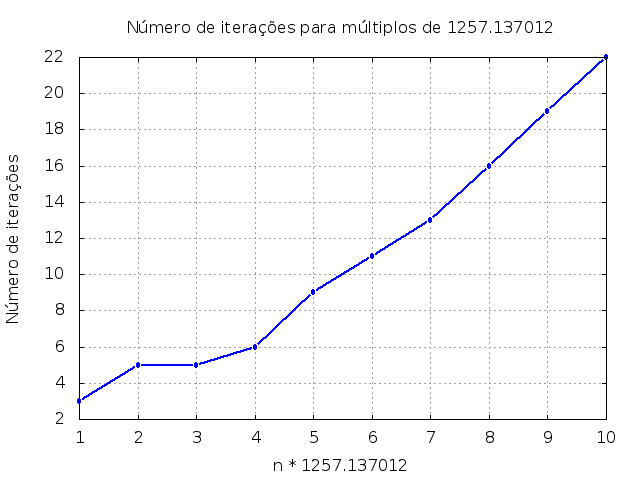
\includegraphics[width=11cm]{../image/questao6.png}
\centering
\caption{Gráfico do número de interações necessárias}
\end{figure}

\paragraph{Questão 7}Para o método da bissecção, com base na mesma estimativa de chute usada para Newton-Rapson, podemos definir um intervalo para $t*$ como sendo $1245<t*<1330$. A partir do qual obteve-se $t*$ com $28$ interações. Assim para um erro  $E = 0.000001$, temos que o número de interações será dado por:
\begin{equation}
n = \frac{ln(t_{max} - t_{min}) -ln (E)}{ln(2)} = 27.34096 \rightarrow n = 28
\end{equation}

\paragraph{Questão 8}Repetindo o processo da questão 6 para valores de x entre 1 e 5 obtemos como curva para a propagação da ``frente de calor'':
\begin{figure}[H]
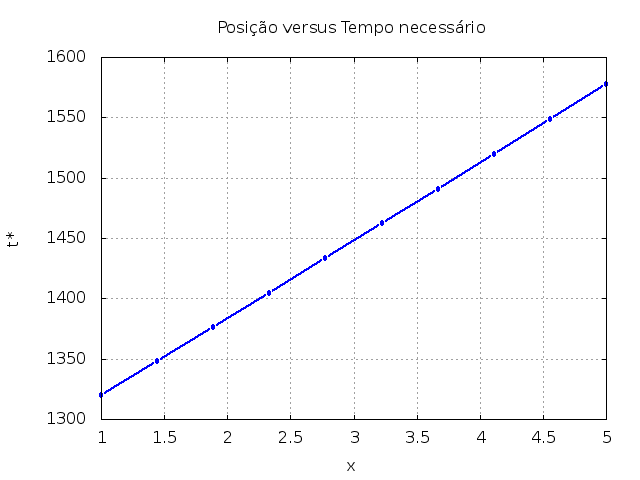
\includegraphics[width=11cm]{../image/questao8.png}
\centering
\caption{Grafíco do número de interações necessárias}
\end{figure}

\paragraph{Questão 9}Avaliando-se os demais parâmetros da função $T(x,t)$, observa-se, tanto para o crescimento de $q$ quanto de $\alpha$ um decaimento exponêncial no tempo necessário para que um ponto $x$ alcance a uma temperatura $T_f$. Tendo sido adotado para o estudo os valores de $x=1$ e $T_f=50$:

\begin{figure}[H]
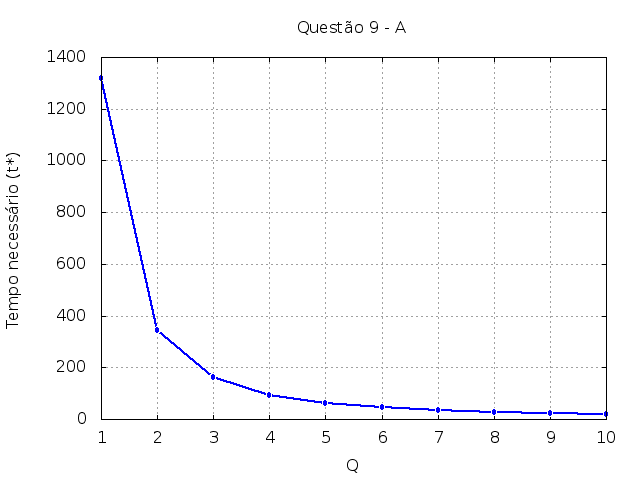
\includegraphics[width=11cm]{../image/questao9a.png}
\centering
\caption{Gráfico de q vs t*}
\end{figure}

\begin{figure}[H]
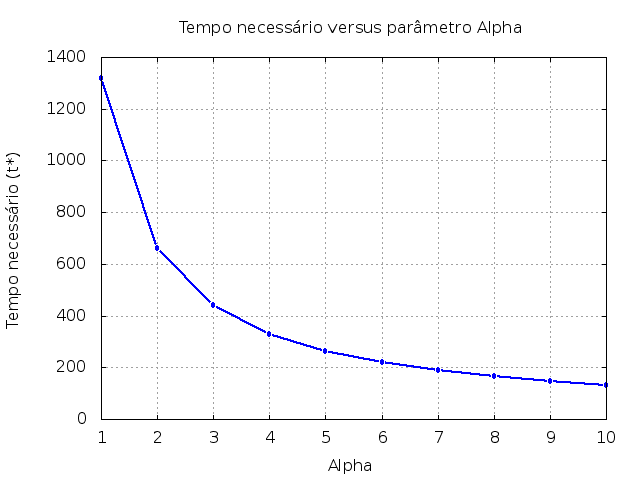
\includegraphics[width=11cm]{../image/questao9b.png}
\centering
\caption{Gráfico de $\alpha$ (A) vs t*}
\end{figure}

\paragraph{}De maneira similar podemos avaliar também a influência de $T_f-T_i$ no tempo $t*$,

\begin{figure}[H]
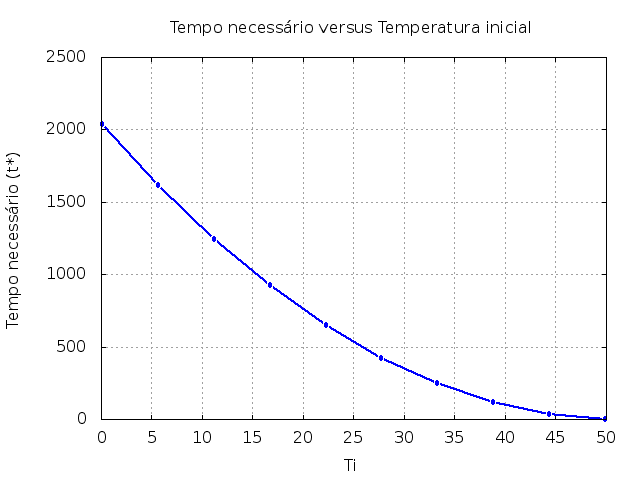
\includegraphics[width=11cm]{../image/questao10.png}
\centering
\caption{Gráfico de $T_f$ vs t*}
\end{figure}

% -------------------------------------------------------------------
\end{document}
